\chapter{Countermeasures}
% \section*{10 - Ottobre}
% \section{Introduction}
\begin{itemize}
    \item \textbf{Proactive} Patching a vulnerability before being vittim of an attack
    \item \textbf{Dynamic} Countermeasure applied during an intrusion to prevent the attacker from reaching its goal e.g. dropping connection
    \item \textbf{Reactive} Patching applied after an intrusion to prevent the success of the next one.
\end{itemize}

\begin{figure}[h]
    \centering
    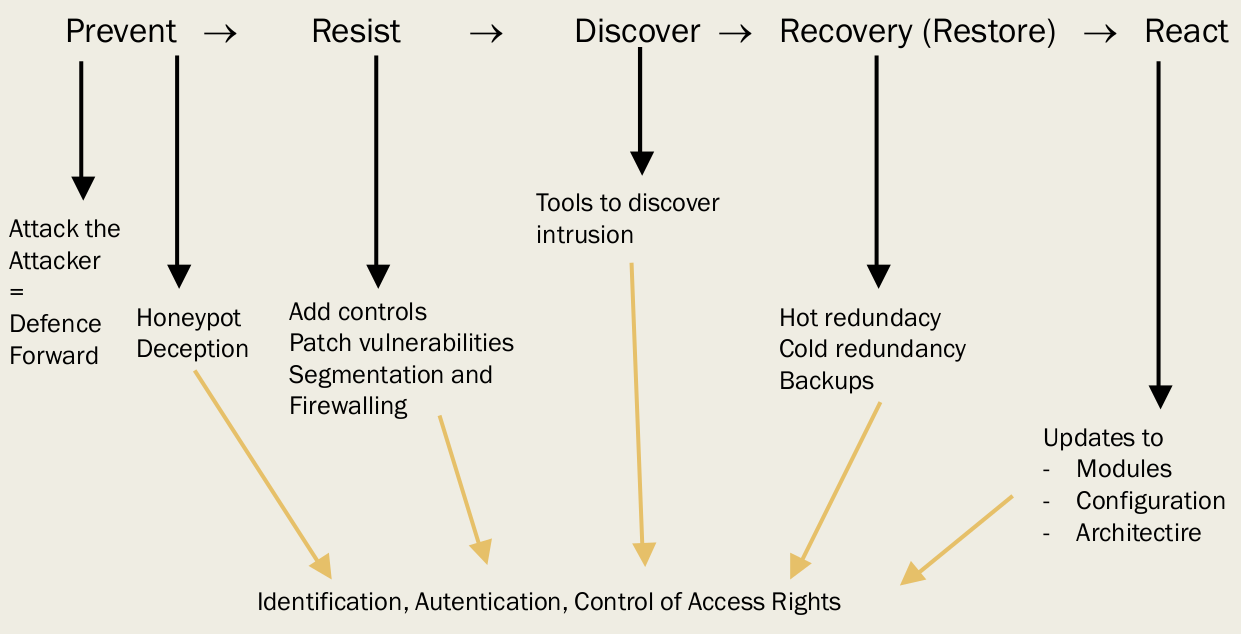
\includegraphics[width=0.6\textwidth]{images/countermeasure_classification.png}
    \caption{Countermeasure more detailed classification}
    \label{fig:countermeasures_classification}
\end{figure}

\section{Robustness and Resilience}
\textbf{Robustness} refers to strength and effectiveness, even in adverse
conditions. The more robust a product is, the less its performance is
affected by disruptions or input changes, because such changes have
been predicted and contingency plans have been developed and built
into the product.

\textbf{Resilience} instead is the ability to bounce back after disruption. Unlike
robustness, which is proactive, resilience is reactive, following
incidents in which system performance has already been affected.
Resilience is measured in terms of the time a system takes to recover
to its original state of performance or better.
\nl
Both can exploit \textbf{redundancy} and \textbf{heterogeneity};
\textbf{heterogeneity} means using modules from distinct suppliers to avoid a catastrophic failure due to a single vulnerability, increasing robustness.\\
\textbf{Redundancy} can clearly highly increase \textit{resilience} to faults,
there are many kinds of redundancy:
\begin{itemize}
    \item \textit{Cold} redundancy: spare and idle instances of modules are started only when working instances are unavailable due to faults or attacks.
    \item \textit{Hot} redundancy: multiple active instances that work simultaneously to tolerate loss due to attack without a recovery e.g. multiple DB copies, or nodes in a network/cloud
    \item \textit{Triple Modular} redundancy: hot redundancy where three instances of a
    module receive the same input, execute the same computation and vote the
    result. Vote can be decentralized or centralized. Space systems use five copies.
    \note{Increases safety but maybe not security}
    \item Overall oversized system in general may allow resource loss
\end{itemize}

Anytime resilience is based upon reconfiguration, system monitoring is fundamental.
System monitoring should discover how close the current system behaviour is close to a boundary and fire the reconfiguration action to remain or return to normal behavior.
The largest the amount of information on the current behavior, the higher the performance of monitoring.

\subsection{Minimal system}
One way of dealing with intrusion is to has a \textbf{minimal system}, i.e. a subset of the system of robut and heterogenous modules,
which can act as a starting point to restore a consistent status.
It is crucial not to lose control on the minimal system,
since doing so might mean not being to restore the normal behaviour.

From this point of view we can also consider a \textbf{minimal behaviour},
i.e. the smallest set of behaviours that is acceptable for the final user.
The minimal behaviour requires some features to ensure robustness which can also be used to restore the normal behaviour after an attack.\\
Consider an ATM and its behaviours as an example, and notice which behaviours compose the {\color{red} minimal} one:
\begin{enumerate}
    \item {\color{red} Protect money}
    \item {\color{red} Interact with a central system}
    \item Distribute money
    \item Distribute information about accounts
\end{enumerate}

\section{Authentication}
\[\langle subject, object, operation \rangle\]
Keeping in mind this triple, there are two kinds of controls which can be done on it; subject \textit{identity} controls and \textit{access rights} ownership controls (i.e. the subject owns the access right).

Most of the mapping of identity into a set of access rights is a task that usually is delegated to the OS,
which can also handle authentication,
but typically specialized components are preferred.

Authentication can be classified as follows:
\begin{itemize}
    \item Weak Static: passwords and similar strategies which can be easily defeated by a sniffing atacker
    \item Weak not Static: cryptographic techniques to produce information that is not repeated
    \item Strong: mathematics and encryption to produce information
    that is not repeated and that may be validated by a distinct
    channel
\end{itemize}

\subsection{Authentication Mechanisms}
\begin{enumerate}
    \item Something the user knows e.g. a password hashed on the server
    \item Something the user owns
    \item Something the user "is" e.g. Biometric Authentication through fingerprint/retina/face
\end{enumerate}

\section{Kerberos}
Strong authentication network protocol
\begin{itemize}
    \item A user password must never travel over the network
    \item must never be stored in any form on the client machine
    \item must be immediately discarded after being used
    \item should never be stored in an unencrypted form even in the authentication database
\end{itemize}
A user enters a password only once per session so that it can transparently access all the
services it is authorized for without having to re-enter the password during this session.
Authentication information management is centralized on the authentication server.
Application servers must not contain authentication information.
Such centralization guarantees no redundancy and possible consistency problems,
allows an admin to perform edits on the auth DB in a one-time action.

Kerberos provides a three-sided authentication with a shared key for \textbf{symmetric encryption}.
The agents are the following:
\begin{enumerate}
    \item Client
    \item Server \note{offers a service but want the users to be authenticated}
    \item KDC Key Distribution Center
    \item TGS TIcket Granting Service
\end{enumerate}
\textbf{Base Principle}: \textit{If you know the shared key then you have been authenticated by the KDS}\\
A \textbf{ticket} allows a client to prove its identity to a server to access the service one offers. 
A ticket is valid in a time window only.\textit{}
However, the \textbf{counterpart }is that centralization introduces both \textit{single-points-of-failure} and potential \textit{performance bottleneck}.\\
Master Keys are encrypted with the \textit{master key} of the \textbf{KDC} and with the one of \textbf{TGS}. The passwords of these two modules are the last line of defence.
\begin{figure}
    \centering
    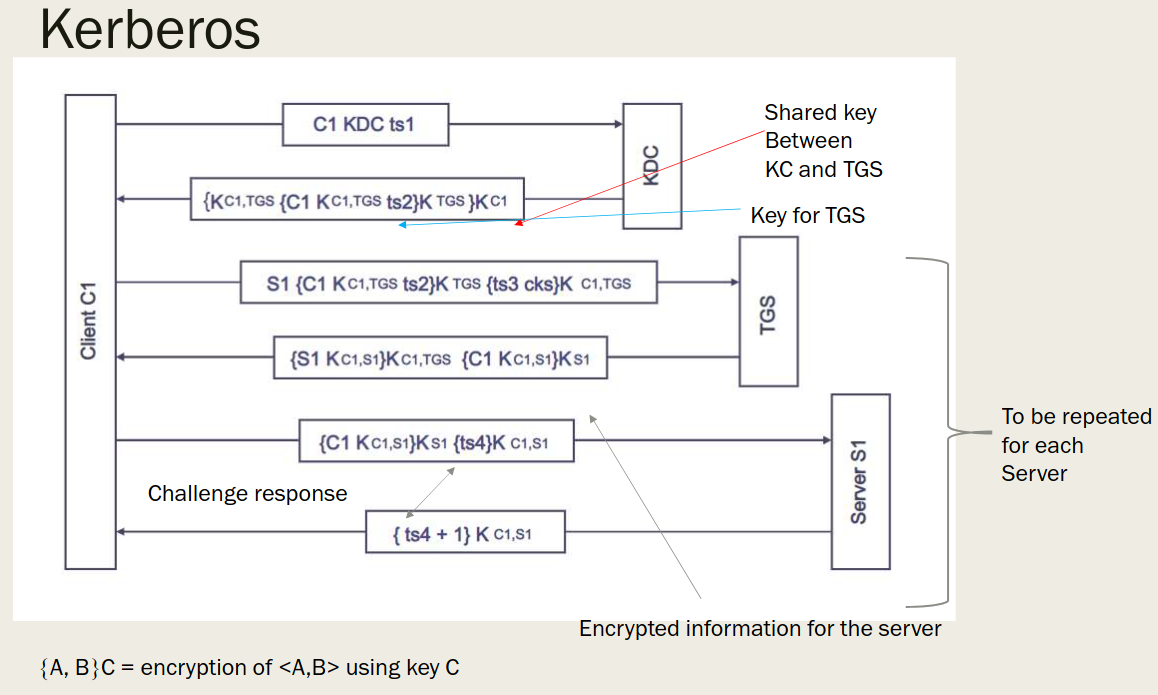
\includegraphics{images/kerberos_messages.png}
    \caption{Kerberos messages exchange}
    \label{fig:kerberos_messages}
\end{figure}

\section{Zero Trust}
A key point of zero trust is that authentication and authorization involve both a subject and a used \textit{device}.
The focus of zero trust is to protect resources instead of network segments since the network
location is no longer seen as the prime component of the security posture of the resource.

\section{Control and Management of Access Rights}
As said before access rights are represented as a matrix which is highly dynamic.\\
Note that any OS has an implementation of this matrix to protect physical resources, logical resources and memory areas.
Besides each application may have its own matrix to protect the resources it manages.

Basically, an OS matrix determines which users can interact with a given application,
and also which operations such users can invoke.

A whole matrix is inefficient due to centralization, thus it is advised to decompose on \textit{rows} or \textit{columns}.

\section{Rows - Capabilities}
A possible implementation is the one with capabilities: this solution stores the access rights in the
subject that then extracts and presents the one that enables the operation of interest.
An example
of usage is the map that translates virtual addresses on physical addresses, each entry in this map
contains some bits that represent the permission for that memory region.

On \textbf{distributed} systems, we need some way to protect capabilities information from tampering because hardware features can’t certify that.
To solve the problem we use a shared secret among the systems and we use that secret as a key to build check digits that are a hash of the capability
produced using the key.
The receiver of the capabilities and of the check digits can use the digits to verify the capability is authentic.\\
In \textbf{centralized} systems, instead, each pointer corresponds to a capability.

\section{Cols - Access Control List}
This solution provides storing the matrix in colums, one column for each object.
An object implementation also stores the information to control the accesses to the object.

An instance of ACL is the packet routing in Linux made with \texttt{iptables},
which allows to define rules for each packet "chain":
\begin{itemize}
    \item Input chain
    \item Output chain
    \item Forward chain
\end{itemize}
Besides it is possible to define default policy PASS/DROP.
For each packet it is possible to perform various actions:
\begin{itemize}
    \item DROP/PASS (route)
    \item goto/return i.e. call/return packet to a chain
    \item Queue i.e. handle packets queue using user's code
    \item Log
    \item Reject
    \item dnat/snat/masquerade
\end{itemize} 

In general, filtering packets going \textit{outside} a node, is called \textbf{egress filtering};
in other words, before allowing an \textit{outbound connection} a user-defined \textit{rule} must be checked.
Such control allows to \textit{discover malware}, stop contributing to \textit{attacks}, or to \textit{block local users} from using illegal services.

\section{Role Based Access Control}
Basically pairing \textit{access rights} with a \textit{professional \textbf{role}}.
When representing such access rights, there is a simple matrix for each role, making room for scalability and easy management.
Clearly, also a mapping between users and roles is needed.

\textit{Roles} may be partially ordered, leading to $R_1,R_2 \Leftrightarrow (R_2.\textit{access\_rights} \in R_1.\textit{access\_rights})$

\section{Attribute Based Access Control}
Access rights are granted or denied according to values of 4 key attributes:
\begin{enumerate}
    \item \textit{\textbf{Subject}}
    \item \textit{\textbf{Action}}
    \item \textit{\textbf{Object}}
    \item \textit{\textbf{Contextual}}
\end{enumerate}

This is a flexible approach, but strongly relies on how attributes resist manipulation.
Besides it must be noted that \textit{ACL} and its derivations can grant access even to unknown subjects,
which instead is not possible with capabilities since they are distributed only to entities we already know.
